% Template of basic phisics experiment 基于 article template, 在此基础上做修改
% 设定文章编码类型, 正文字号为五号则 zihao=5, 正文字号为小四则 zihao=-4
\documentclass[zihao=5, UTF8]{article}


% 自定义宏定义
\def\N{\mathbb{N}}
\def\F{\mathbb{F}}
\def\Z{\mathbb{Z}}
\def\Q{\mathbb{Q}}
\def\R{\mathbb{R}}
\def\C{\mathbb{C}}
\def\T{\mathbb{T}}
\def\S{\mathbb{S}}
\def\A{\mathbb{A}}
\def\I{\mathscr{I}}
\def\d{\mathrm{d}}
\def\p{\partial}


% 物理实验报告所需的其它宏包
\usepackage{ulem}   % \uline 下划线支持

% 导入基本宏包
\usepackage[UTF8]{ctex}     % 设置文档为中文语言
\usepackage[colorlinks, linkcolor=blue, anchorcolor=blue, citecolor=blue, urlcolor=blue]{hyperref}  % 宏包: 自动生成超链接 (此宏包与标题中的数学环境冲突)
% \usepackage{docmute}    % 宏包: 子文件导入时自动去除导言区, 用于主/子文件的写作方式, \include{./51单片机笔记}即可. 注: 启用此宏包会导致.tex文件capacity受限.
\usepackage{amsmath}    % 宏包: 数学公式
\usepackage{physics}
\usepackage{bm}
\usepackage{mathrsfs}   % 宏包: 提供更多数学符号
\usepackage{amssymb}    % 宏包: 提供更多数学符号
\usepackage{pifont}     % 宏包: 提供了特殊符号和字体
\usepackage{extarrows}  % 宏包: 更多箭头符号
\usepackage{multirow}
\usepackage{siunitx}

\renewcommand{\dd}{\mathrm{d}}

% 列表环境设置
\usepackage{enumitem}   % 宏包: 列表环境设置
    \setlist[enumerate]{itemsep=0pt, parsep=0pt, topsep=0pt, partopsep=0pt, leftmargin=3.5em}
    \setlist[itemize]{itemsep=0pt, parsep=0pt, topsep=0pt, partopsep=0pt, leftmargin=3.5em}
    \newlist{circledenum}{enumerate}{1} % 创建一个新的枚举环境
    \setlist[circledenum,1]{
        label=\protect\circled{\arabic*}, % 使用 \arabic* 来获取当前枚举计数器的值, 并用 \circled 包装它
        ref=\arabic*, % 如果需要引用列表项, 这将决定引用格式(这里仍然使用数字)
        itemsep=0pt, parsep=0pt, topsep=0pt, partopsep=0pt, leftmargin=3.5em
    }
% 文章页面 margin 设置
\usepackage[a4paper]{geometry}  % 宏包: 文章页面 margin 设置
    \geometry{top=0.75in}
    \geometry{bottom=0.75in}
    \geometry{left=0.75in}
    \geometry{right=0.75in}   % 设置上下左右页边距
    \geometry{marginparwidth=1.75cm}    % 设置边注距离(注释、标记等)

% 自定义数学环境
\usepackage{amsthm} % 宏包: 数学环境配置
% theorem-line 环境自定义
    \newtheoremstyle{MyLineTheoremStyle}% <name>
        {11pt}% <space above>
        {11pt}% <space below>
        {}% <body font> 使用默认正文字体
        {}% <indent amount>
        {\bfseries}% <theorem head font> 设置标题项为加粗
        {: }% <punctuation after theorem head>
        {.5em}% <space after theorem head>
        {\textbf{#1}\thmnumber{#2}\ \ (\,\textbf{#3}\,)}% 设置标题内容顺序
    \theoremstyle{MyLineTheoremStyle} % 应用自定义的定理样式
    \newtheorem{LineTheorem}{Theorem.\,}
% theorem-block 环境自定义
    \newtheoremstyle{MyBlockTheoremStyle}% <name>
        {11pt}% <space above>
        {11pt}% <space below>
        {}% <body font> 使用默认正文字体
        {}% <indent amount>
        {\bfseries}% <theorem head font> 设置标题项为加粗
        {: \\ \indent}% <punctuation after theorem head>
        {.5em}% <space after theorem head>
        {\textbf{#1}\thmnumber{#2}\ \ (\,\textbf{#3}\,)}% 设置标题内容顺序
    \theoremstyle{MyBlockTheoremStyle} % 应用自定义的定理样式
    \newtheorem{BlockTheorem}[LineTheorem]{Theorem.\,} % 使用 LineTheorem 的计数器
% definition 环境自定义
    \newtheoremstyle{MySubsubsectionStyle}% <name>
        {11pt}% <space above>
        {11pt}% <space below>
        {}% <body font> 使用默认正文字体
        {}% <indent amount>
        {\bfseries}% <theorem head font> 设置标题项为加粗
        {: \\ \indent}% <punctuation after theorem head>
        {0pt}% <space after theorem head>
        {\textbf{#3}}% 设置标题内容顺序
    \theoremstyle{MySubsubsectionStyle} % 应用自定义的定理样式
    \newtheorem{definition}{}


% 有色文本框及其设置
\usepackage[dvipsnames,svgnames]{xcolor}    %设置插入的文本框颜色
\usepackage[strict]{changepage}     % 提供一个 adjustwidth 环境
\usepackage{framed}     % 实现方框效果
    \definecolor{graybox_color}{rgb}{0.95,0.95,0.96} % 文本框颜色. 修改此行中的 rgb 数值即可改变方框纹颜色, 具体颜色的rgb数值可以在网站https://colordrop.io/ 中获得. (截止目前的尝试还没有成功过, 感觉单位不一样)(找到喜欢的颜色, 点击下方的小眼睛, 找到rgb值, 复制修改即可)
    \newenvironment{graybox}{%
    \def\FrameCommand{%
    \hspace{1pt}%
    {\color{gray}\small \vrule width 2pt}%
    {\color{graybox_color}\vrule width 4pt}%
    \colorbox{graybox_color}%
    }%
    \MakeFramed{\advance\hsize-\width\FrameRestore}%
    \noindent\hspace{-4.55pt}% disable indenting first paragraph
    \begin{adjustwidth}{}{7pt}%
    \vspace{2pt}\vspace{2pt}%
    }
    {%
    \vspace{2pt}\end{adjustwidth}\endMakeFramed%
    }

% 各级标题自定义设置
\usepackage{titlesec}
    % section标题自定义设置
    \titleformat{\section}[hang]{\normalfont\huge\bfseries\centering}{第\,\thesection\,部分}{20pt}{}
    % subsection标题自定义设置
    \titleformat{\subsection}[hang]{\normalfont\Large\bfseries}{\,\thesubsection\,}{8pt}{}
    % subsubsection标题自定义设置
    \titleformat{\subsubsection}[hang]{\normalfont\large\bfseries}{\,\thesubsubsection\,}{6pt}{}

% 外源代码插入设置
\usepackage{matlab-prettifier}
    \lstset{
        style=Matlab-editor,  % 继承matlab代码颜色等
    }
\usepackage[most]{tcolorbox} % 引入tcolorbox包
\usepackage{listings} % 引入listings包
    \tcbuselibrary{listings, skins, breakable}
    \lstdefinestyle{matlabstyle}{
        language=Matlab,
        basicstyle=\small,
        breakatwhitespace=false,
        breaklines=true,
        captionpos=b,
        keepspaces=true,
        numbers=left,
        numbersep=15pt,
        showspaces=false,
        showstringspaces=false,
        showtabs=false,
        tabsize=2
    }
    \newtcblisting{matlablisting}{
        arc=0pt,
        top=0pt,
        bottom=0pt,
        left=1mm,
        listing only,
        listing style=matlabstyle,
        breakable,
        colback=white   % 选一个合适的颜色
    }

% table 支持
\usepackage{booktabs}   % 宏包: 三线表
\usepackage{tabularray} % 宏包: 表格排版
\usepackage{longtable}  % 宏包: 长表格

% figure 设置
\usepackage{graphicx}  % 支持 jpg, png, eps, pdf 图片
\usepackage{svg}       % 支持 svg 图片
    \svgsetup{
        % 指向 inkscape.exe 的路径
        inkscapeexe = C:/aa_MySame/inkscape/bin/inkscape.exe,
        % 一定程度上修复导入后图片文字溢出几何图形的问题
        inkscapelatex = false
    }


% 图表进阶设置
\usepackage{float}     % 图表位置浮动设置
\usepackage{caption}    % 图注、表注
    \captionsetup[figure]{name=图}
    \captionsetup[table]{name=表}
    \captionsetup{labelfont=bf, font=small}

%% 文章默认字体设置
%    \usepackage{fontspec}   % 宏包: 字体设置
%        \setmainfont{SimSun}[
%            BoldFont = SimHei, % 设置粗体字为黑体
%            ItalicFont = KaiTi, % 设置斜体字为楷体
%            BoldItalicFont = KaiTi % 设置粗斜体字为楷体
%        ]
%        %\setCJKmainfont[AutoFakeBold=3]{SimSun} % 设置加粗字体为 SimSun 族, AutoFakeBold 可以调整字体粗细
%        \setmainfont{Times New Roman} % 设置英文字体为Times New Roman


% 其它设置
    % equation 公式编号设置
        \makeatletter
        \renewcommand{\theequation}{\thesection.\arabic{equation}}
        \makeatother
    % 脚注设置
        \renewcommand\thefootnote{\ding{\numexpr171+\value{footnote}}}
    % 参考文献引用设置
        \bibliographystyle{unsrt}   % 设置参考文献引用格式为unsrt
        \newcommand{\upcite}[1]{\textsuperscript{\cite{#1}}}     % 自定义上角标式引用
    % 文章序言设置
        \newcommand{\cnabstractname}{序言}
        \newenvironment{cnabstract}{%
            \par\Large
            \noindent\mbox{}\hfill{\bfseries \cnabstractname}\hfill\mbox{}\par
            \vskip 2.5ex
            }{\par\vskip 2.5ex}


% 页眉页脚设置
\usepackage{fancyhdr}   %宏包: 页眉页脚设置
    \pagestyle{fancy}
    \fancyhf{}
    \cfoot{\thepage}
    \renewcommand\headrulewidth{1pt}
    \renewcommand\footrulewidth{0pt}
    \rhead{\bfseries 分组序号: 3-04-1}
    \chead{《基础物理实验》实验报告,\ 潘天麟\ 2023K8009908023}
    \lhead{2024.12.18}

\usepackage{pdfpages}

% 开始编辑文章

\begin{document}
\noindent\begin{flushright}
    \zihao{2}{分组序号: 3-04-1}
\end{flushright}

\newcommand*{\boldsong}{\CJKfamily{boldsong}}


\begin{center}\large
    \noindent{\Huge\bfseries\boldsong《基础物理实验》实验报告 }
    \\\vspace{0.4cm}
    \noindent\textit{
        \textbf{\boldsong 实验名称: }\uline{\hspace{2.3cm} 磁滞回线\hspace{2.3cm}}\hspace{0.4cm}
        指导教师: \uline{\hspace{1.5cm} 郭志英 \hspace{1.5cm}}}
    \\\vspace{0.1cm}
    \noindent\textit{
        姓名: \uline{\,\,潘天麟\,\,}\hspace{0.2cm}
        学号: \uline{\,\,{\upshape 2023K8009908023}\,\,}\hspace{0.2cm}
        专业: \uline{\,\,人工智能\,\,}\hspace{0.2cm}
        班级: \uline{\,\,\upshape{2313}\,\,}\,组号: \uline{\,\,\upshape{3-04-1}\,\,}}
    \\\vspace{0.1cm}
    \noindent\textit{
        实验日期: \uline{\,\,{\upshape 2024.12.18}\,\,}\hspace{0.2cm}
        实验地点: \uline{\,\,\,教学楼{\upshape 713}\,\,\,}\hspace{0.2cm}
        是否调课/补课: \uline{\,\,否\,\,}\hspace{0.2cm}
        成绩: \uline{\hspace{2cm}}}
\end{center}
% \vspace{-0.2cm}
\noindent\rule{\textwidth}{0.1em}   % 分割线

% 控制目录不换页
\vspace{1cm}
\setcounter{tocdepth}{3}  % 目录深度为 2(不显示 subsubsection)
\noindent\begin{minipage}{\textwidth}\centering
\tableofcontents\thispagestyle{fancy}   % 显示页码、页眉等
\end{minipage}
\newpage

\section{实验目的}
\begin{enumerate}
    \item 掌握利用示波器测量铁磁材料动态磁滞回线的方法. 
    \item 掌握利用霍尔传感器测量铁磁材料 (准) 静态磁滞回线的方法. 
    \item 了解铁磁性材料的磁化特性. 
    \item 了解磁滞、磁滞回线和磁化曲线的概念, 加深对饱和磁化强度、剩余磁化强度、矫顽力等物理量的理解. 
\end{enumerate}

\section{实验仪器}
\begin{itemize}
    \item DH4516磁特性综合测量实验仪 (包括正弦波信号源, 待测样品及绕组, 积分电路所用的电阻和电容) . 示波器, 直流电源, 电感. 
    \begin{enumerate}
        \item  样品1：锰锌铁氧体, 圆形罗兰环, 磁滞损耗较小. 平均磁路长度$l = 0.130$ m, 铁芯实验样品截面积$S = 1.24 \times 10^{-4}$ m$^2$, 选取匝数：$N_1 = 150$, $N_2 = 150$, $N_3 = 150$. 
        \item  样品2：EI型硅钢片, 磁滞损耗较大. 平均磁路长度$l = 0.075$ m, 铁芯实验样品截面积 $S = 1.20 \times 10^{-4}$ m$^2$, 线圈匝数：$N_1 = 150$, $N_2 = 150$, $N_3 = 150$. 
        \item  信号源的频率在20~200 Hz间可调; 可调标准电阻$R_1$,$R_2$均为无感交流电阻, $R_1$的调节范围为$0.1 \sim 11$ Ω; $R_2$的调节范围为$1 \sim 110$ kΩ.  标准电容有$0.1 \sim 11$ μF可选. 
    \end{enumerate}
    \item FD-BH-I 磁性材料磁滞回线和磁化曲线测定仪 (包括数字式特斯拉计、恒流源、磁性材料样品、磁化线圈、双刀双掷开关、霍耳探头移动架、双叉头连接线、箱式实验平台) . 
    
    \begin{enumerate}
        \item  数字式特斯拉计：四位半 LED 显示, 量程 2.000T; 分辨率 0.1mT; 带霍耳探头. 
        \item  恒流源：四位半 LED 显示, 可调恒定电流 0-600.0mA. 
        \item  磁性材料样品：条状矩形结构, 截面长 2.00cm; 宽 2.00cm; 隔隙 2.00mm; 平均磁路长度=0.240m (样品与固定螺丝为同种材料) . 
        \item  磁化线圈总匝数 $N=2000$. 
    \end{enumerate}
\end{itemize}

\section{实验原理}
将物体放在外磁场H中, 物体就会被磁化, 内部产生磁场. 记物体内部的磁化强度为M, 磁感应强度为B, 则物体的磁化率$\chi_m$和相对磁导率$\mu_r$定义为
\begin{equation}
\chi_m=M/H
\end{equation}
\begin{equation}
\mu_r=B/(\mu_0 H)=(\mu_0 (B+H))/(\mu_0 H)=\chi_m+1
\end{equation}
根据磁化率可以将物质分为抗磁性物质、铁磁性物质和顺磁性物质3种. 抗磁性物质的磁化率为负值, 通常在$10^{-5}$~$10^{-6}$量级, 且几乎不随温度变化; 顺磁性物质的磁化率通常在$10^{-4}$~$10^{-4}$量级, 且随温度线性增大; 而铁磁性物质的磁化率通常大于1, 且随温度增高而减小. 
除了磁导率高以外, 铁磁材料还具有特殊的磁化规律. 对一个处于磁中性状态的铁磁材料加上由小变大的磁场H进行磁化时, 磁感应强度B随H的变化曲线称为起始磁化曲线, 大致可分为可逆磁化阶段、不可逆磁化阶段和饱和磁化阶段. 在可逆磁化阶段, 减小H, 则B会沿原路径返回原点; 在不可逆磁化阶段, 若减小H, 则B不会沿原路线返回原点, 呈现图1中的回路形式; 在饱和磁化阶段, 继续增大H, B不继续增大, 而由于$B=\mu_0 (B+H)$, B会随着H线性增大, 但增量极小. 途中$H_s$和$B_s$分别称为饱和磁场强度和饱和磁感应强度. 
\begin{figure}[H]
    \centering
    
\includegraphics[width=0.5\textwidth]{fig1.png}
    \caption{铁磁材料的起始磁化曲线和饱和磁滞回线示意图}
    \label{fig:1} 
\end{figure}

若将铁磁材料磁化到饱和状态, 如图\ref{fig:1}中的S点, 再减小磁场H, 那么磁感应强度B会随着H的减小而减小, 但并不沿起始磁化曲线SAO减小, 而是沿着SP减小. 当H减小到0时, B并不为0, 此时的磁感应强度称为剩余磁感应强度$B_r$; 增大反向磁场强度, 可使B继续减小, B为0时的磁场强度为$-H_c$, $H_c$称为矫顽力; 继续增大反向磁场强度, B从0开始反向增大直至$-B_s$, 此时外磁场强度达到$-H_s$, 铁磁材料达到反向饱和磁化状态S'. 若H从反向饱和值$-H_s$变化到0再增大至$H_s$时, B会沿曲线S'P'Q'S返回至正向饱和值$B_s$. 曲线S'P'Q'S与SPQS'关于原点中心对称, 它们形成的闭合曲线SPQS'P'Q'S称为饱和磁滞回线. 
由于铁磁材料加上磁场H后产生的B与磁化历史也有关, 所以再研究铁磁材料的起始磁化性质时, 需要对铁磁材料进行退磁处理, 使之达到磁中性状态. 可以对铁磁材料进行交流退磁, 即对材料施加交变磁化场, 先用大幅度励磁电流使其饱和磁化, 再缓慢改变励磁电流幅度至0使其退磁. 
若磁场在任意$[-H_m,H_m ]$范围内循环变化, 则B也会做循环变化, 形成一个闭合的磁滞回线, 磁滞回线的面积对应于循环磁化一周所发生的能量损耗. 对材料进行准静态磁化时, 损耗来自于磁滞损耗. 对材料进行交流动态磁化时, 除了由磁滞损耗外, 还会有涡流损耗和剩余损耗. 一般由金属和合金所组成的金属磁性材料电阻率低, 在高频磁化时其涡流损耗大, 而由金属氧化物组成的铁氧体磁性材料电阻率高, 高频条件下其涡流损耗很小. 
在同一频率下, 交变磁场幅度不同时, 动态磁滞回线也会不同. 将磁场幅值从0增到$H_s$, 这些动态磁滞回线的顶点($H_m,B_m$)的连线称为动态磁化曲线, 如图\ref{fig:2}. 在这条线上任意一点$B_m$和对应的$H_m$的比值
\begin{equation}
\mu_m=B_m/(\mu_0 H_m)
\end{equation}
称为振幅磁导率. 振幅磁导率是衡量工作在幅度较大的交变磁场下的电感铁芯性能的一个重要指标. 

\begin{figure}[H]
    \centering
    
\includegraphics[width=0.5\textwidth]{fig2.png}
    \caption{铁磁材料的动态磁滞回线和动态磁化曲线示意图}
    \label{fig:2}
\end{figure}

当交流磁化场幅度很小时, 铁磁材料的磁化过程是可逆的, 磁滞回线退化成一条斜线 (如图\ref{fig:2}中原点附近的小线段) . 对于没有直流偏置磁场的情况, 这个过程对应于起始磁化曲线起始的可逆阶段 (图\ref{fig:1}中的OA段) , 定义起始磁导率$\mu_i$为
\begin{equation}
\mu_i=\lim_{H\rightarrow 0}B/(\mu_0 H)
\end{equation}
它表征了起始可逆磁化阶段的磁化性能. 
	有的电感铁芯工作在既有直流偏置又有交流弱磁场的情况下, 比如在图\ref{fig:1}中的D点附近以弱交变磁场循环磁化, 当磁场足够弱时回线会退化成一条斜线, 此时, 交流弱磁场引起的磁感应强度变化$\Delta B$与磁场强度变化值$\Delta H$之比决定了电感性能, 定义可逆磁导率$\mu_R$为
\begin{equation}
\mu_R=\lim_{\Delta H\rightarrow 0}\Delta B/(\mu_0 \Delta H)
\end{equation}
测量动态磁滞回线的原理电路如图\ref{fig:3}所示：

\begin{figure}[H]
    \centering
    
\includegraphics[width=0.5\textwidth]{fig3.png}
    \caption{用示波器测量动态磁滞回线电路图}
    \label{fig:3}
\end{figure}
铁芯上有三层线圈, N1为交流励磁线圈, N2为感应线圈, N3为直流励磁线圈, 在N1处接交流电流源, 则磁场中的磁场强度正比于电流强度也正比于R1上的电压强度, N2处接RC积分电路, 磁感应强度正比于C上的电压强度, 将u1与uc接入示波器, 在x-y模式下就可以观测到动态磁滞回线
由安培环路定理, 
\begin{equation}
Hl=N_1 i_1
\end{equation}
其中$N_1$为线圈1的匝数, l为磁环的等效磁路长度, 由欧姆定理
\begin{equation}
i_1=u_{R_1 }/R_1
\end{equation}
联立两式可得
\begin{equation}
H=N_1/(R_1 l) u_{R_1 }
\end{equation}
即H与$u_{R_1 }$成正比. 由法拉利电磁感应定律
\begin{equation}
u_2=-N_2  d\Phi/dt=-N_2 S dB/dt
\end{equation}
其中$N_2$是线圈2的匝数, $\Phi$为单匝线圈的磁通量, S为单匝线圈环绕的面积. 若$R_2 C\gg T$(T为外磁场周期), 则电容C上的电压远小于总电压$u_2$, 满足
\begin{equation}
u_c=Q/C=1/C \int i_2 dt=1/(CR_2 ) \int u_{R_2 } dt \approx 1/(CR_2 ) \int u_2 dt
\end{equation}
其中Q为电容器极板上的电荷量, $i_2$为线圈2中的电流. 联立 (9) ,  (10) 式可得
\begin{equation}
B=(R_2 C)/(N_2 S) u_c
\end{equation}
如果对绕上磁化线圈的铁磁材料样品施加直流激励, 便会在样品中产生稳定的磁场. 当直流激励的大小发生变化, H与B也随之改变, 形成磁化曲线和磁滞回线. 如果在样品的磁路中开一极窄均匀气隙, 在对磁化线圈中的磁化电流最大值$I_m$磁锻炼的基础上, 对应每个磁化电流$I_k$值, 用数字式特斯拉计, 测量气隙均匀磁场区中间部位的磁感应强度B, 便能得到该磁性材料的磁滞回线.  

\begin{figure}[H]
    \centering
    
\includegraphics[width=0.5\textwidth]{fig4.png}
    \caption{ (左) 磁化曲线和此致曲线,  (右) 基本磁化曲线}
    \label{fig:4}
\end{figure}

用霍尔传感器测量静态磁滞回线的原理电路如图\ref{fig:5}所示：

\begin{figure}[H]
    \centering
    
\includegraphics[width=0.5\textwidth]{fig5.png}
    \caption{磁滞回线和磁化曲线测量装置}
    \label{fig:5}
\end{figure}

其中通过电流表得出励磁电流大小, 通过数字式特斯拉计读出磁感应强度B的大小, 通过反向开关来交换电流方向. 
每次测量前需要对样品进行退磁, 为了得到稳定的磁滞回线, 需要对样品进行反复磁锻炼, 进而保证励磁电流大小不变. 
由安培环路定理：
\begin{equation}
H = N / \overline{l} I
\end{equation}
考虑到样品间缝隙的存在对其进行修正后, 得到：
\begin{equation}
H\overline{l} + H_g l_g = NI
\end{equation}
在$l_g$极小的情况下, 有：
\begin{equation}
B_g S_g=BS, \quad B_g = u_0 u_r H_g
\end{equation}
经过修正后, 得到的式子为：
\begin{equation}
H\overline{l} + (Bl_g)/u_0=NI
\end{equation}

\section{实验内容}

\subsection{观测样品1 (铁氧体) 的饱和动态磁滞回线}
\begin{enumerate}
    \item 将正弦信号波源的频率调为$f=100$ Hz. 取$R_1=2.0\,\Omega$, $R_2=50$ k$\Omega$, $C=10.0\,\mu$F. 示波器选择X-Y模式. 调节励磁电流大小及示波器的垂直, 水平位移旋钮, 在示波器显示屏上调出一个相对于原点对称的饱和磁滞回线, 测量并画出饱和磁滞回线的B-H图. 上下半支各选取7个测量点, 测量$B_s,B_r,H_c$. 通过示波器光标进行读数. 
    \item 保持信号源幅度不变, 在仪器频率可调范围内, 观测不同频率时的饱和磁滞回线. 保持$R_1,R_2,C$不变, 测量并比较$f=95$ Hz和$150$ Hz时的$B_r$和$H_c$.
    \item 将正弦信号波源的频率调为$f=50$ Hz, 固定励磁电流幅度$I_m=0.1$ A, $R_1=2.0\,\Omega$. 依次调节$R_2=50$ k$\Omega$, $5$ k$\Omega$, $1$ k$\Omega$, 使$R_2C$分别为$0.5$ s, $0.05$ s和$0.01$ s. 
\end{enumerate}

\subsection{观测样品1 (铁氧体) 的动态磁滞回线}
\begin{enumerate}
    \item 对铁氧体样品进行退磁处理, 改变正弦信号波源的频率, 测量并画出动态磁化曲线. 取$R_1=2.0\,\Omega$, $R_2=50$ k$\Omega$, $C=10.0\,\mu$F. 磁场幅度$H_m$从$0$到$H_s$单调增加. 
    \item 根据测量数据计算并画出$\mu_m$-$H_m$曲线. 
    \item 测定起始磁导率$\mu_i$. 
\end{enumerate}

\subsection{观察不同频率下样品2 (硅钢) 的动态磁滞回线}
\begin{enumerate}
    \item 对硅钢样品进行退磁处理, 取$R_1=2.0\,\Omega$, $R_2=50$ k$\Omega$, $C=10.0\,\mu$F. 在给定交变磁场幅度$H_m=400$ A/m下, 测量$f=20$ Hz, $40$ Hz, $60$ Hz的$B_m$, $B_r$, $H_c$. 
\end{enumerate}

\subsection{测量样品1 (铁氧体) 在不同直流偏置磁场$H$下的可逆磁导率}
\begin{enumerate}
    \item 对铁氧体样品进行退磁处理, 交流磁场频率取$f=100$ Hz. 电路参数设置为$R_1=2.0\,\Omega$, $R_2=20$ k$\Omega$, $C=2.0\,\mu$F. 直流偏置磁场从$0$到$H_s$单调增加. 测量时调节交流信号源幅度使交流磁场$\Delta H$足够小, 并调节示波器使李萨如图形充分放大. 画出$\mu_R$-$H$曲线. 
\end{enumerate}
\subsection{测量样品的起始磁化曲线}
\begin{enumerate}
    \item 将样品退磁处理后, 改变$I$的大小, 测量不同$I$下的$B$值大小, 测量B-H关系曲线
\end{enumerate}

\subsection{测量模具钢的磁滞回线}
\begin{enumerate}
    \item 将模具钢进行磁锻炼后, 将$I$逐步减小到$0$, 再将$I$反向到最大值, 再从反向最大值回归到$0$, 最后再从$0$到正向最大值, 测量不同$I$下的$B$
\end{enumerate}

\section{实验数据及处理}
\subsection{观测样品1 (铁氧体) 的饱和动态磁滞回线}
\begin{table}[H]
    \centering
    \begin{tabular}{|c|c|c|} 
    \hline
    $H$(mV) & $B$(数据点1)(mV) & $B$(数据点2)(mV)  \\ 
    \hline
    209   & 20.2        & 20.2         \\ 
    \hline
    68    & 13.6        & 15.6         \\ 
    \hline
    18    & 8.4         & 0            \\ 
    \hline
    0     & 3.6         & -4.8         \\ 
    \hline
    -12   & 0           & -8.1         \\ 
    \hline
    -48   & -9.6        & -13.2        \\ 
    \hline
    -212  & -20          & -20           \\
    \hline
    \end{tabular}
    \caption{铁氧体的饱和动态磁滞回线数据}
    \label{tab:1}
\end{table}

根据\ref{tab:1}中的数据, 利用$H = N_1/(R_1 l) u_{R_1}$和$B=(R_2 C)/(N_2 S) u_c$, 可以得到铁氧体的饱和动态磁滞回线如图\ref{fig:plot1}所示：

\begin{figure}[H]
    \centering
    
\includegraphics[width=0.8\textwidth]{plot1.pdf}
    \caption{铁氧体的饱和动态磁滞回线}
    \label{fig:plot1}
\end{figure}

其中正半轴的矫顽力为$H_{c1} = 10.38 \unit{A/m}$, 负半轴的矫顽力为$H_{c2} = 6.92 \unit{A/m}$, 正半轴的剩余磁感应强度为$B_{r1} = 96.77 \unit{mT}$,
负半轴的剩余磁感应强度为$B_{r2} = 129.03 \unit{mT}$, 正半轴的饱和磁感应强度为$B_{s1} = 543.01 \unit{mT}$, 负半轴的饱和磁感应强度为$B_{s2} = 537.63 \unit{mT}$

保持$R_1,R_2,C$不变, 测量并比较$f=95$ Hz和$150$ Hz时的$B_r$和$H_c$, 如表\ref{tab:2}所示：
\begin{table}[H]
\centering
\begin{tabular}{|c|c|c|}
    \hline
    mV    & 95 Hz & 150 Hz \\
    \hline
    $B_r$ & 4.8 & 2.5 \\
    \hline
    $H_c$ & 20 & 8 \\
    \hline
\end{tabular}
\caption{不同频率下的铁氧体的$B_r$和$H_c$}
\label{tab:2}
\end{table}

可以观察到的现象是, 当励磁电流的频率升高时, 磁性材料的磁滞回线会缩小. 这表现为剩磁 ($B_r$) 和矫顽力 ($H_c$) 均减小, 并且磁滞回线所包围的面积也随之减小. 

\begin{align*}
    &\textbf{当频率升高时：} & \textbf{当频率降低时：}\\
    &\text{励磁线圈的自感电动势 } \uparrow & \text{励磁线圈的自感电动势 } \downarrow \\
    &\text{线圈上的有效电压 } (u_{R_1})  \downarrow  & \text{线圈上的有效电压 } (u_{R_1})  \uparrow  \\
    &\text{磁化电流} (i_1) \downarrow & \text{磁化电流} (i_1) \uparrow \\
     &\text{磁场强度} (H_m = N i_1) \downarrow  & \text{磁场强度} (H_m = N i_1) \uparrow  \\
    &\text{剩磁 } (B_r) \downarrow & \text{剩磁 } (B_r) \uparrow \\
    &\text{矫顽力 } (H_c) \downarrow & \text{矫顽力 } (H_c) \uparrow \\
    & \text{磁滞回线缩小} &  \text{磁滞回线扩大}
\end{align*}

这种现象背后的机理是, 励磁线圈本身具有电感特性. 频率的升高会导致线圈中产生更大的自感电动势, 该电动势会反向抵消电源的驱动电压. 这导致线圈上的有效电压 ($u_{R_1}$) 减小, 从而减小流过线圈的电流 ($i_1$), 进而减小磁化磁场 $H_m$. 磁化磁场的减小导致较小的 $B_r$ 和较小的磁滞回线面积. 当频率降低时, 则发生相反的情况. 实验数据证实, 随着频率的增加, 计算得到的 $B_r$ 值会减小, 这验证了上述描述的关系. 

~\\

接着, 我们保持频率不变, 取$R_1=2.0\,\Omega$, $R_2=50$ k$\Omega$, $C=10.0\,\mu$F, 依次调节$R_2=50$ k$\Omega$, $5$ k$\Omega$, $1$ k$\Omega$, 使$R_2C$分别为$0.5$ s, $0.05$ s和$0.01$ s. 得到的李萨如图形如图\ref{fig:6}所示：

% three figures in one row using minipage
\begin{figure}[H]
    \centering
    \begin{minipage}[b]{0.3\textwidth}
        \centering
        
\includegraphics[width=0.98\textwidth]{fig6.jpg}
        \caption*{$R_2C=0.01$ s}
    \end{minipage}
    \begin{minipage}[b]{0.3\textwidth}
        \centering
        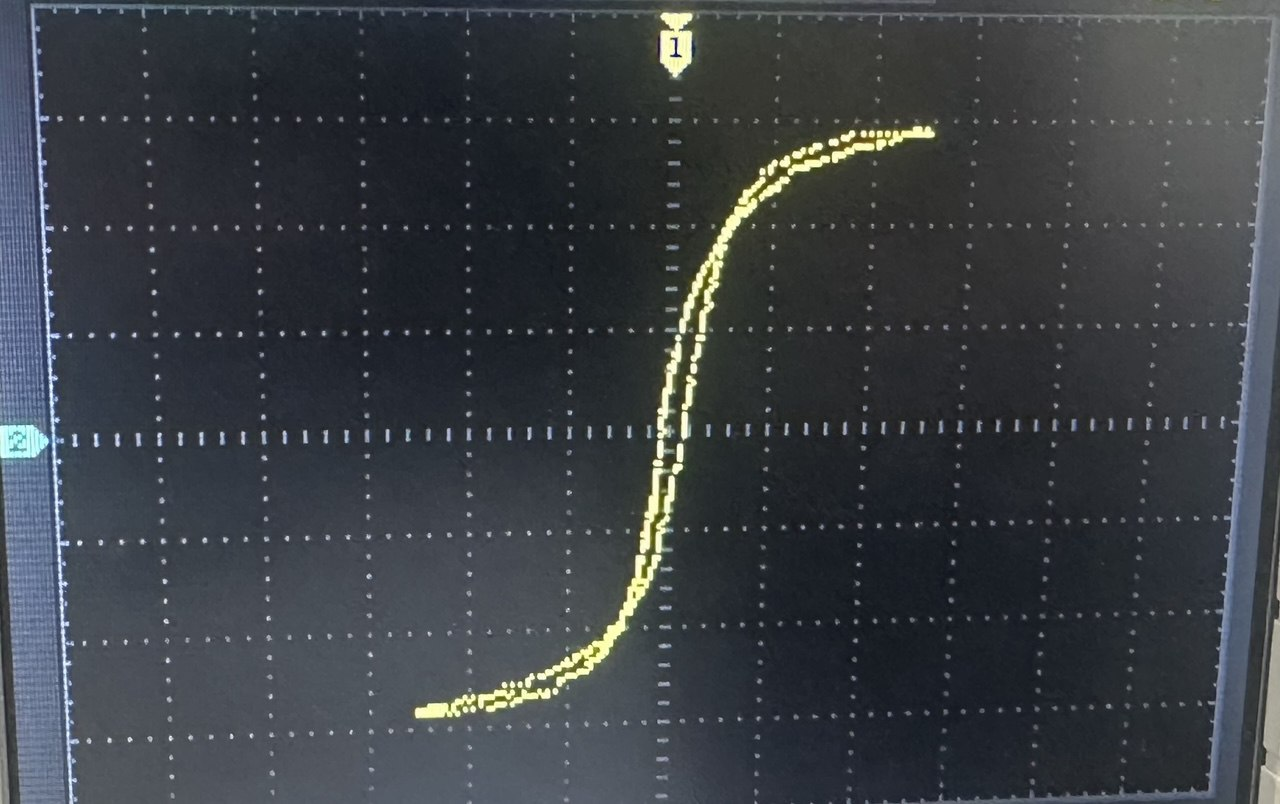
\includegraphics[width=\textwidth]{fig7.jpg}
        \caption*{$R_2C=0.05$ s}
    \end{minipage}
    \begin{minipage}[b]{0.3\textwidth}
        \centering
        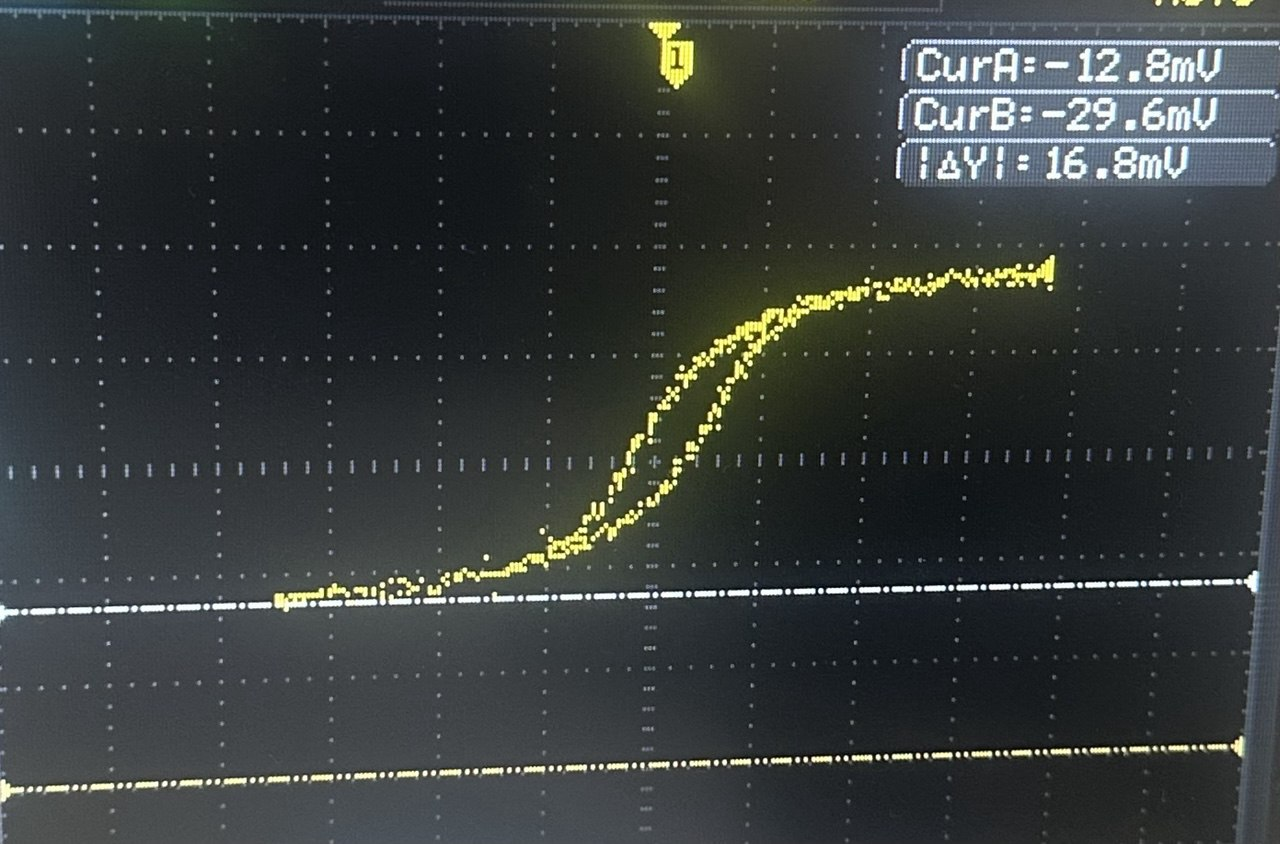
\includegraphics[width=0.96\textwidth]{fig8.jpg}
        \caption*{$R_2C=0.5$ s}
    \end{minipage}
    \caption{不同$R_2C$下的李萨如图形}
    \label{fig:6}
\end{figure}

为了解释积分常数对李萨如图形 (由 $u_{R_1}$ 和 $u_c$ 形成) 的影响, 考虑到其中$u_c$ 的计算依赖于近似 $\frac{1}{CR_2}\int u_{R_2} dt \approx \frac{1}{CR_2}\int u_2 dt$, 此近似成立的前提是时间常数 $R_2C$ 远大于测量周期 $T$ ($\ensuremath{R_2C\gg T}$). 若此条件不满足, 则 $u_{R_2}$ 和 $u_2$ 之间的差异不可忽略, 导致 $u_c$ 的计算误差, 并影响 $u_c$ 与磁场强度 $B$ 之间的线性关系 ( $B= \frac{R_2C}{N_2S}u_c $) , 体现为李萨如图形的变化. 然而, 由于积分常数仅影响 $u_c $ 的计算, 不影响最终的 $B$ 值, 因此积分常数对实际的 $B-H$ 磁滞回线形状不会产生影响. 因此, 在测量中, 只有当满足 $R_2C\gg T$ 时, 才能准确地通过测量电容电压 $u_c$ 来计算磁场强度 $B$. 

\subsection{观测样品1 (铁氧体) 的动态磁化曲线}

\begin{table}[H]
\centering
\begin{tabular}{|c|c|c|c|c|c|c|c|c|c|c|} 
\hline
mV     & 1    & 2    & 3    & 4    & 5    & 6    & 7    & 8    & 9    & 10    \\ 
\hline
($H_m$) & 0    & 5.36 & 6.24 & 9.12 & 13.8 & 20.8 & 25.6 & 33.6 & 48   & 58.9  \\ 
\hline
($B_m$) & 0    & 1.60  & 1.96 & 2.94 & 5.4  & 6.8  & 7.8  & 9.6  & 12   & 13.2  \\ 
\hline
mV     & 11   & 12   & 13   & 14   & 15   & 16   & 17   & 18   & 19   & 20    \\ 
\hline
($H_m$) & 70   & 82   & 104  & 118  & 132  & 148  & 156  & 170  & 182  & 202   \\ 
\hline
($B_m$) & 14.8 & 15.2 & 16   & 16.8 & 16.8 & 17.2 & 17.2 & 17.6 & 17.6 & 18    \\
\hline
\end{tabular}
\caption{铁氧体的动态磁滞回线数据}
\label{tab:3}
\end{table}

根据\ref{tab:3}中的数据, 利用$H = N_1/(R_1 l) u_{R_1}$和$B=(R_2 C)/(N_2 S) u_c$, 可以得到铁氧体的动态磁滞回线如图\ref{fig:plot2}所示：

\begin{figure}[H]
    \centering
    
\includegraphics[width=0.8\textwidth]{plot2.pdf}
    \caption{铁氧体的动态磁化曲线}
    \label{fig:plot2}
\end{figure}

再根据$\mu_m=B_m/(\mu_0 H_m)$, 可以得到铁氧体的$\mu_m$-$H_m$曲线如图\ref{fig:plot3}所示：

\begin{figure}[H]
    \centering
    
\includegraphics[width=0.8\textwidth]{plot3.pdf}
    \caption{铁氧体的$\mu_m$-$H_m$曲线}
    \label{fig:plot3}
\end{figure}

用多项式拟合的结果为
\begin{equation}
    \mu_m = -7.427 \times 10^{-8} H_m^6
    + 2.925 \times 10^{-5} H_m^5
    - 4.505 \times 10^{-3} H_m^4
    + 0.340 H_m^3
    - 12.59 H_m^2
    + 150.8 H_m
    + 4204 
\end{equation}

由此得到的起始磁导率$\mu_i$为$4204$, 这和4000左右的理论值是相符的. 

\subsection{观察不同频率下样品2 (硅钢) 的动态磁滞回线}
\begin{table}[H]
\centering
\begin{tabular}{|c|c|c|c|} 
\hline
mV & 20 Hz & 40 Hz & 60 Hz  \\ 
\hline
$B_m$ & 32.8  & 32.6  & 32.8   \\ 
\hline
$B_r$ & 19.6  & 24    & 23.2   \\ 
\hline
$H_c$ & 128   & 132   & 144    \\
\hline
\end{tabular}
\caption{硅钢的动态磁滞回线数据(原始)}
\label{tab:4}
\end{table}

由表\ref{tab:4}中的数据可以发现, 随着频率的增加, $H_c$有明显的增大, 但是$B_m$和$B_r$的变化趋势则不是很明显.
我们可以由此推断$H_c$和频率有关.

\subsection{测量样品1 (铁氧体) 在不同直流偏置磁场下的可逆磁导率}
\begin{table}[H]
    \centering
    \begin{tabular}{|c|c|c|c|c|c|c|c|c|c|c|} 
    \hline
    电流 (A) & 0.01 & 0.02 & 0.03 & 0.04 & 0.05 & 0.06 & 0.07 & 0.08 & 0.09 & 0.1   \\ 
    \hline
    $\Delta H$ (A/m)     & 2.88 & 3.4  & 4.4  & 6.48 & 8.88 & 11.2 & 13.6 & 15.2 & 16.4 & 16.8  \\ 
    \hline
    $\Delta B$ (mT)    & 4.2  & 4.8  & 5.2  & 4.6  & 4.6  & 4.4  & 4.2  & 3.4  & 2.8  & 2.2   \\
    \hline
    \end{tabular}
    \caption{铁氧体的可逆磁导率数据}
    \label{tab:5}
\end{table}

利用$\mu_R = \lim_{\Delta H \to 0} \frac{\Delta B}{\mu_0 \Delta H}$
和$Hl = N_1 i_1$, 可以得到\ref{tab:6}中的数据

\begin{table}[H]
\centering
\begin{tabular}{|c|c|c|c|c|c|c|c|c|c|c|} 
\hline
$H$ (A/m)     & 11.53 & 23.08  & 34.61  & 46.15 & 57.69 & 69.23 & 80.77 & 92.31 & 103.85 & 115.38  \\ 
\hline
$\mu_R$    & 4642  & 4467  & 3761  & 2288  & 1649  & 1251  & 983  & 712  & 543  & 417   \\
\hline
\end{tabular}
\caption{铁氧体的可逆磁导率数据(计算)}
\label{tab:6}
\end{table}

根据表\ref{tab:6}中的数据, 可以得到铁氧体的$\mu_R$-$H$曲线如图\ref{fig:plot4}所示：

\begin{figure}[H]
    \centering
    
\includegraphics[width=0.8\textwidth]{plot4.pdf}
    \caption{铁氧体的$\mu_R$-$H$曲线}
    \label{fig:plot4}
\end{figure}

\subsection{测量样品的起始磁化曲线}
\begin{table}[H]
    \centering
    \begin{tabular}{|c|c|c|c|c|c|c|c|} 
    \hline
    $I$ (mA) & $B$ (mT) & $H$ (A/m) & 修正 $H$ (A/m) & $I$ (mA) & $B$ (mT) & $H$ (A/m) & 修正 $H$ (A/m)  \\ 
    \hline
    0      & 0      & 0.0     & 0.0        & 300.7  & 148.0  & 2505.8  & 1563.6      \\ 
    \hline
    30     & 7.1    & 250.0   & 204.8      & 330.0  & 168.2  & 2750.0  & 1679.2      \\ 
    \hline
    59.9   & 15.0   & 499.2   & 403.7      & 360.0  & 188.7  & 3000.0  & 1798.7      \\ 
    \hline
    90.4   & 23.5   & 753.3   & 603.7      & 390.2  & 209.1  & 3251.7  & 1920.5      \\ 
    \hline
    120.0  & 36.5   & 1000.0  & 767.6      & 419.9  & 228.7  & 3499.2  & 2043.2      \\ 
    \hline
    149.9  & 51.7   & 1249.2  & 920.0      & 449.9  & 247.5  & 3749.2  & 2173.5      \\ 
    \hline
    180.0  & 68.0   & 1500.0  & 1067.1     & 480.3  & 265.7  & 4002.5  & 2311.0      \\ 
    \hline
    210.5  & 85.9   & 1754.2  & 1207.3     & 510.3  & 285.2  & 4252.5  & 2436.9      \\ 
    \hline
    240.8  & 106.8  & 2006.7  & 1326.8     & 540.1  & 298.3  & 4500.8  & 2601.8      \\ 
    \hline
    269.9  & 126.7  & 2249.2  & 1442.6     & 571.0  & 313.6  & 4758.3  & 2761.9      \\
    \hline
    \end{tabular}
    \caption{样品的起始磁化曲线数据}
    \label{tab:7}
\end{table}

根据表\ref{tab:7}中的数据, 可以得到样品的起始磁化曲线如图\ref{fig:plot5}所示：

\begin{figure}[H]
    \centering
    
\includegraphics[width=0.8\textwidth]{plot5.pdf}
    \caption{样品的起始磁化曲线}
    \label{fig:plot5}
\end{figure}

\subsection{测量模具钢的磁滞回线}

\begin{table}[H]
\centering
\begin{tabular}{|c|c|c|c|c|c|c|c|} 
\hline
$I$ (mA) & $B$ (mT) & $H$ (A/m) & 修正 $H$ (A/m) & $I$ (mA) & $B$ (mT) & $H$ (A/m) & 修正 $H$ (A/m)  \\ 
\hline
600.1  & 333.5  & 5000.8  & 2877.7    & -600   & -339.5 & -5000.0 & -2838.7    \\ 
\hline
550.9  & 329.0  & 4590.8  & 2496.4    & -550.3 & -332.8 & -4585.8 & -2467.2    \\ 
\hline
499.3  & 321.1  & 4160.8  & 2116.6    & -500.6 & -325.2 & -4171.7 & -2101.4    \\ 
\hline
449.7  & 311.9  & 3747.5  & 1761.9    & -450.3 & -316.2 & -3752.5 & -1739.5    \\ 
\hline
400.3  & 300.7  & 4160.8  & 2246.5    & -399.2 & -305.1 & -3326.7 & -1384.3    \\ 
\hline
349.3  & 286.2  & 2910.8  & 1088.8    & -349.5 & -291.7 & -2912.5 & -1055.5    \\ 
\hline
300.5  & 268.6  & 2504.2  & 794.2     & -299.9 & -274.7 & -2499.2 & -750.4     \\ 
\hline
250.2  & 245.6  & 2085.0  & 521.5     & -249.7 & -253.0 & -2080.8 & -470.2     \\ 
\hline
199.5  & 217.4  & 1662.5  & 278.5     & -200.3 & -226.7 & -1669.2 & -225.9     \\ 
\hline
149.9  & 185.9  & 1249.2  & 65.7      & -149.6 & -195.5 & -1246.7 & -2.1       \\ 
\hline
100.1  & 151.1  & 834.2   & -127.8    & -100.1 & -162.3 & -834.2  & 199.1      \\ 
\hline
50.6   & 116.9  & 421.7   & -322.5    & -49.7  & -126.5 & -414.2  & 391.2      \\ 
\hline
0      & 78.3   & 0.0     & -498.5    & 0      & -89.7  & 0.0     & 571.0      \\ 
\hline
-50.4  & 39.6   & -420.0  & -672.1    & 50.6   & -51.0  & 421.7   & 746.3      \\ 
\hline
-100.3 & 0.5    & -835.8  & -839.0    & 100.5  & -12.3  & 837.5   & 915.8      \\ 
\hline
-150.1 & -38.8  & -1250.8 & -1003.8   & 150.5  & 27.1   & 1254.2  & 1081.6     \\ 
\hline
-200.7 & -78.5  & -1672.5 & -1172.8   & 200.2  & 66.0   & 1668.3  & 1248.2     \\ 
\hline
-250.7 & -116.3 & -2089.2 & -1348.8   & 249.8  & 103.5  & 2081.7  & 1422.8     \\ 
\hline
-299.9 & -152.6 & -2499.2 & -1527.7   & 301.6  & 141.9  & 2513.3  & 1610.0     \\ 
\hline
-349.8 & -188.5 & -2915.0 & -1715.0   & 350.4  & 176.9  & 2920.0  & 1793.8     \\ 
\hline
-400.1 & -223.4 & -3334.2 & -1912.0   & 400.8  & 212.1  & 3340.0  & 1989.7     \\ 
\hline
-459.3 & -256.4 & -3827.5 & -2195.2   & 450.3  & 244.5  & 3752.5  & 2196.0     \\ 
\hline
-500.0 & -286.9 & -4166.7 & -2340.2   & 500.0  & 274.7  & 4166.7  & 2417.9     \\ 
\hline
-550.3 & -314.8 & -4585.8 & -2581.8   & 550.4  & 302.2  & 4586.7  & 2662.8     \\ 
\hline
-600.0 & -339.5 & -5000.0 & -2838.7   & 600.4  & 326.2  & 5003.3  & 2926.7     \\
\hline
\end{tabular}
\caption{模具钢的磁滞回线数据}
\label{tab:8}
\end{table}

根据表\ref{tab:8}中的数据, 可以得到模具钢的磁滞回线如图\ref{fig:plot6}所示：

\begin{figure}[H]
    \centering
    
\includegraphics[width=0.8\textwidth]{plot6.pdf}
    \caption{模具钢的磁滞回线}
    \label{fig:plot6}
\end{figure}

由此可以得到$B_m = 339.5 \unit{mT}$, $H_m = 5003.3 \unit{A/m}$, $H_c = 840 \unit{A/m}$

\section{实验讨论}
本次实验中, 我们通过测量铁氧体和硅钢的磁滞回线, 动态磁化曲线, 可逆磁导率, 起始磁化曲线, 以及模具钢的磁滞回线, 得到了这些材料的磁性参数. 通过这些参数, 我们可以了解这些材料的磁性特性, 以及不同频率, 不同直流偏置磁场下的磁性特性. 

实验产生的数据量较大, 需要处理的数据较多, 我们可以合理使用OCR工具来快速识别手写的数据, 并利用Python等工具进行数据处理, 以提高实验效率.

在测量铁氧体的动态磁化曲线时, 我发现当外场强度较低时, 示波器的成像质量不是很好, 噪声角度, 且较难用光标读取我们感兴趣的数据. 我尝试过更换连接示波器的BMC线, 但是效果并不是很好. 后来我又发现, 在测量时有手摁住BMC线的连接处, 示波器的成像质量会有所提高. 这可能是由于连接处的接触不良导致的, 在以后的实验中, 我们可以更换连接线, 或者更换示波器, 以提高实验效果.

实验采用的光标读取数据的办法精度并不高, 尤其是在噪声比较多的情况下, 我们不知道需要让光标具体指向哪个点. 在以后的实验中, 我们可以尝试使用更加精确的数据处理方法, 比如说将示波器的数据导出到电脑上, 利用专业的数据处理软件进行去噪后, 再计算出可信的磁滞回线端点等特殊点的坐标.

在计算起始磁导率时, 我发现最后的计算结果和拟合方式的选取有很大关系. 我认为这是因为我们在小磁场强度下的数据点较少, 较难拟合出一个合理的曲线. 但是也正如前文所说小磁场下示波器的的误差较大, 所以为了得到一个更加准确的结果, 有必要使用更加精确的测量仪器.

\section{思考题}
\textbf{铁磁材料的动态磁滞回线与 (准) 静态磁滞回线在概念上有什么区别? 铁磁材料动态磁滞回线的形状和面积受那些因素影响? }
~\\
\begin{itemize}
    \item 动态磁滞回线：当磁场在两个方向上来回变化时, 介质磁化过程所形成的$B-H$闭合曲线. 这意味着磁场的变化速度足够快, 材料的磁化过程可能无法及时响应, 导致磁滞回线的形状发生变化. 
    \item 静态 (或准静态) 磁滞回线：在缓慢变化的磁场 (准静态过程) 下, 铁磁材料的磁化过程所形成的$B-H$闭合曲线. 这意味着磁场的变化足够慢, 材料的磁化时刻处于平衡状态. 
\end{itemize}
动态磁滞回线的形状和面积受以下因素影响:
\begin{itemize}
    \item 材料特性:
    \begin{itemize}
        \item 材料的成分和晶体结构: 不同的材料具有不同的磁化特性. 
        \item 材料的形状和体积: 较小的样品可能表现出不同的磁化行为. 
    \end{itemize}
    \item 外部条件:
    \begin{itemize}
        \item 温度: 温度会影响材料的磁化能力. 
        \item 磁化场的幅度: 磁场强度的大小会影响磁滞回线的形状. 
        \item 磁化场的频率: 磁场变化的频率越高, 磁滞损耗通常越大, 回线形状也可能发生变化. 
    \end{itemize}
\end{itemize}

\textbf{什么叫做基本磁化曲线? 它和起始磁化曲线间有何区别? }
~\\
基本磁化曲线是一系列大小不同的磁滞回线的顶点连接而成的一条曲线, 它不要求铁磁体的最初状态是未被磁化的. 

\textbf{铁氧体和硅钢材料的动态磁化特性各有什么特点? }
~\\
铁氧体的磁滞损耗小, 因此在动态磁化过程中, 硅钢材料的剩余磁感应强度和矫顽力都比铁氧体的大. 

\textbf{动态磁滞回线测量实验中, 电路参量应怎样设置才能保证所形成的李萨如图形正确反映材料动态磁滞回线的形状? }
~\\
为了使李萨如图形准确反映材料的动态磁滞回线, 测试电路的时间常数 ($R_2C$) 必须远大于激励信号的周期 (T) . 即:$ R_2C >> T $. 这样可以确保积分电路的输出电压能够真实地表示磁感应强度 (B) . 如果$R_2C$与$T$相当或更小, 则输出可能失真, 不能真实反映材料的磁滞回线. 

\textbf{准静态磁滞回线测量实验中, 为什么要对样品进行磁锻炼才能获得稳定的饱和磁滞回线? }
~\\
因为对样品进行磁锻炼之后模具钢的磁化性质会更加稳定. 

\section{附录}
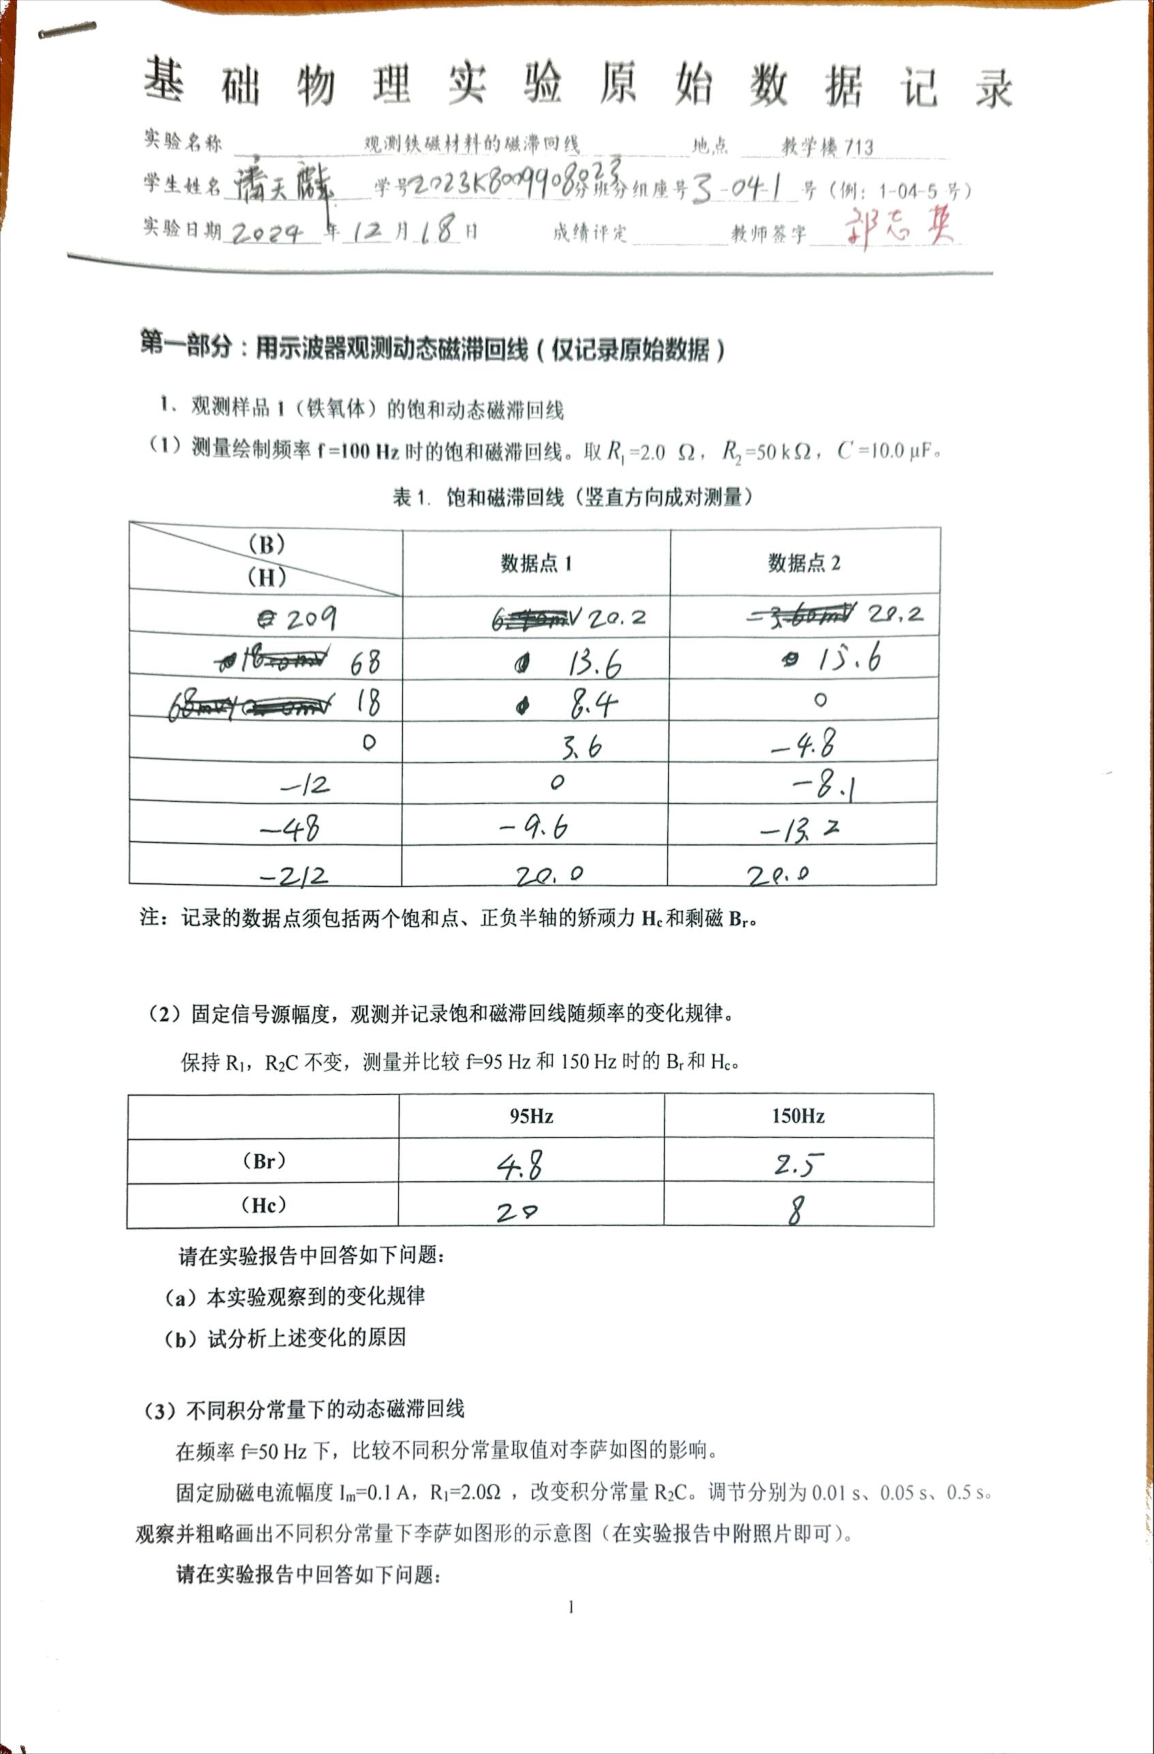
\includepdf[pages=-]{潘天麟-磁滞回线-数据.pdf}
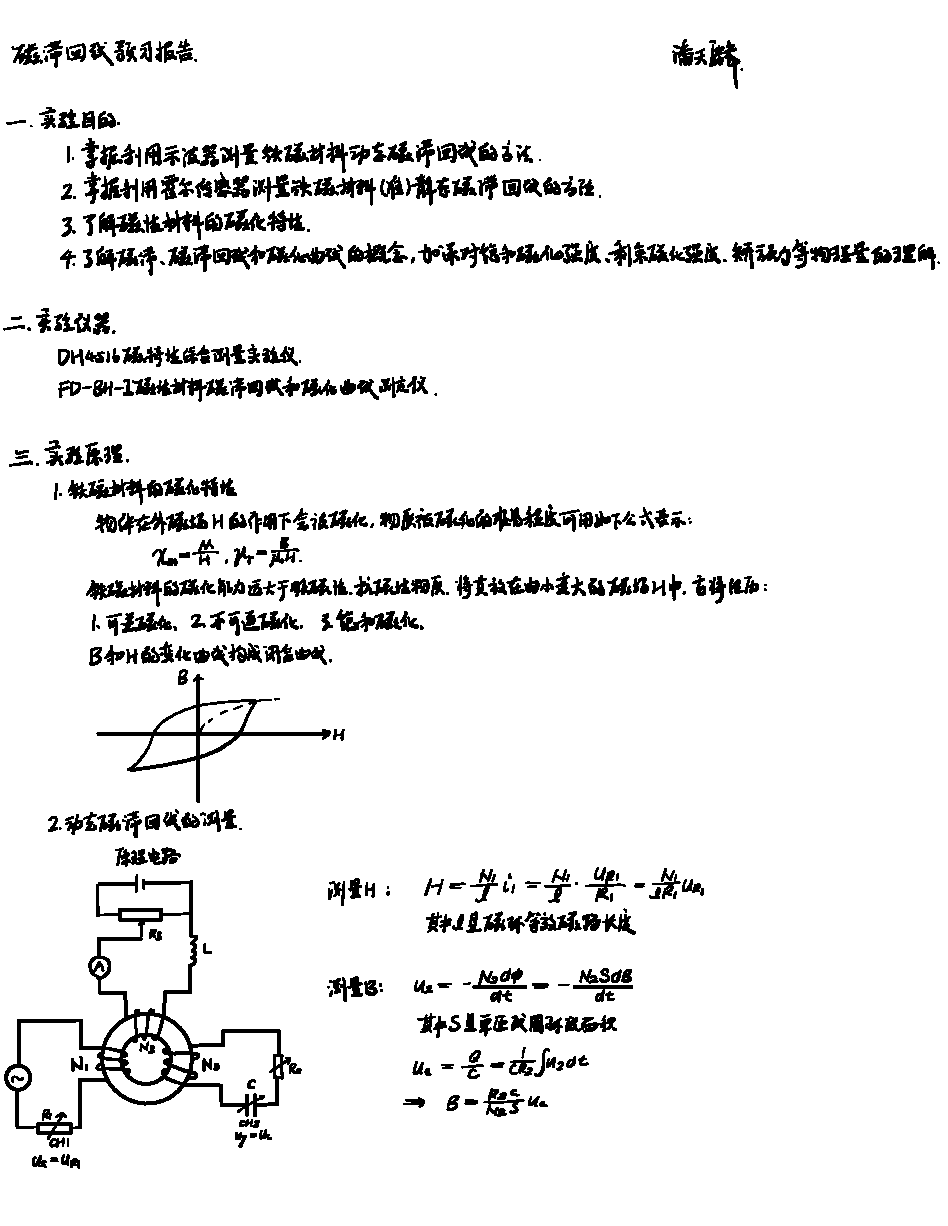
\includepdf[pages=-]{潘天麟-2024-12-18-磁滞回线-预习报告.pdf}
\end{document}
